\documentclass{standalone}

\usepackage[utf8]{inputenc}
\usepackage{amsfonts}
\usepackage{amssymb,amsmath}
\usepackage{tikz}

\begin{document}

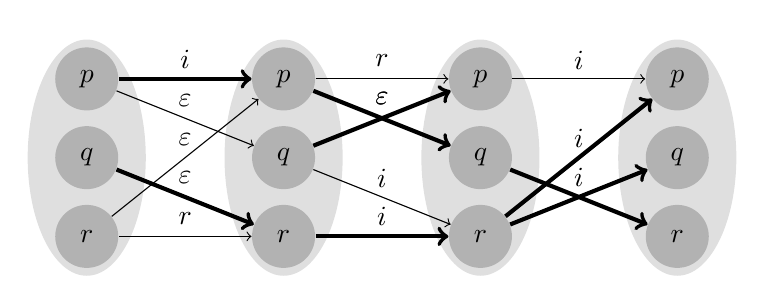
\begin{tikzpicture}[every node/.style={circle,inner sep=0pt,minimum size = .8cm}]
    \fill[gray!25] (0,0) ellipse (0.75 and 1.5);
    \fill[gray!25] (2.5,0) ellipse (0.75 and 1.5);
	\fill[gray!25] (5,0) ellipse (0.75 and 1.5);
 	\fill[gray!25] (7.5,0) ellipse (0.75 and 1.5);

%	\node at (0,2) {$0$};
%	\node at (2.5,2) {$1$};
%	\node at (5,2) {$2$};
%	\node at (7.5,2) {$3$};

%	\node at (10.5,1.5) {\begin{huge}$\cdots$\end{huge}};
%	\node at (10.5,0) {\begin{huge}$\cdots$\end{huge}};
%	\node at (10.5,-1.5) {\begin{huge}$\cdots$\end{huge}};

	\node[fill=gray!60] (p1) at (0,1) {$p$};
	\node[fill=gray!60] (q1) at (0,0) {$q$};
	\node[fill=gray!60] (r1) at (0,-1) {$r$};

	\node[fill=gray!60] (p2) at (2.5,1) {$p$};
	\node[fill=gray!60] (q2) at (2.5,0) {$q$};
	\node[fill=gray!60] (r2) at (2.5,-1) {$r$};

	\node[fill=gray!60] (p3) at (5,1) {$p$};
	\node[fill=gray!60] (q3) at (5,0) {$q$};
	\node[fill=gray!60] (r3) at (5,-1) {$r$};

	\node[fill=gray!60] (p4) at (7.5,1) {$p$};
	\node[fill=gray!60] (q4) at (7.5,0) {$q$};
	\node[fill=gray!60] (r4) at (7.5,-1) {$r$};

  \draw[->] (p1) edge [line width=1.5pt] node[above=-5pt] {$i$} (p2);
  \draw[->] (p1) edge node[above=-5pt] {$\varepsilon$} (q2);
  \draw[->] (q1) edge [line width=1.5pt] node[above=-5pt] {$\varepsilon$} (r2);
  \draw[->] (r1) edge node[above=-5pt] {$\varepsilon$} (p2);
  \draw[->] (r1) edge node[above=-5pt] {$r$} (r2);

  \draw[->] (p2) edge node[above=-5pt] {$r$} (p3);
  \draw[->] (p2) edge [line width=1.5pt] node[above=-5pt] {$\varepsilon$} (q3);
  \draw[->] (q2) edge [line width=1.5pt] node[above=-5pt] {$\varepsilon$} (p3);
  \draw[->] (q2) edge node[above=-5pt] {$i$} (r3);
  \draw[->] (r2) edge [line width=1.5pt] node[above=-5pt] {$i$} (r3);
	
  \draw[->] (p3) edge node[above=-5pt] {$i$} (p4);
  \draw[->] (q3) edge [line width=1.5pt] node[above=-5pt] {$i$} (r4);
  \draw[->] (r3) edge [line width=1.5pt] node[above=-5pt] {$i$} (p4);
  \draw[->] (r3) edge [line width=1.5pt] node[above=-5pt] {} (q4);
\end{tikzpicture}

\end{document}
